\begin{center}
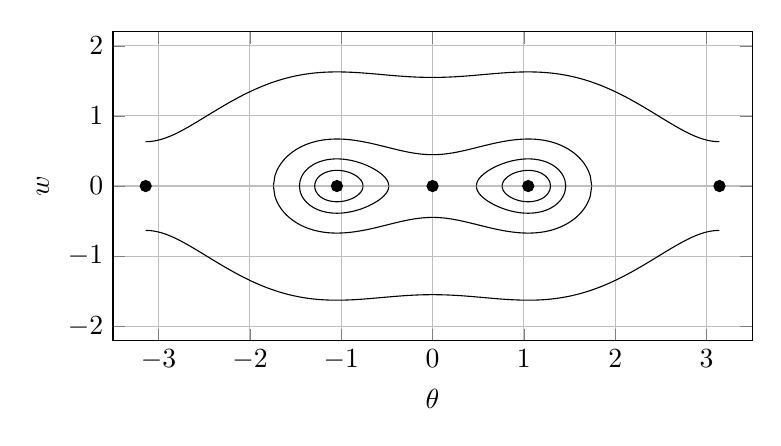
\begin{tikzpicture}
\begin{axis}[width=.8\textwidth,height=5.5cm,xlabel={$\theta$},ylabel={$w$},xmin=-3.5,xmax=3.5,ymin=-2.2,ymax=2.2,grid=major]
% Each plotted interval is physically allowed; max only suppresses endpoint rounding.
\foreach \en in {-.1,-.05}{
\pgfmathsetmacro{\lo}{acos((1+sqrt(1+8*\en))/2)*pi/180}
\pgfmathsetmacro{\hi}{acos((1-sqrt(1+8*\en))/2)*pi/180}
\foreach \sgn in {-1,1}{
\addplot[no marks,domain=\lo:\hi,samples=150]{\sgn*sqrt(max(0,2*(\en-.5*cos(deg(x))^2+.5*cos(deg(x)))))};
\addplot[no marks,domain=-\hi:-\lo,samples=150]{\sgn*sqrt(max(0,2*(\en-.5*cos(deg(x))^2+.5*cos(deg(x)))))};}
}
\pgfmathsetmacro{\turn}{acos((1-sqrt(1.8))/2)*pi/180}
\foreach \sgn in {-1,1}{
\addplot[no marks,domain=-\turn:\turn,samples=220]{\sgn*sqrt(max(0,2*(.1-.5*cos(deg(x))^2+.5*cos(deg(x)))))};
\addplot[no marks,domain=-pi:pi,samples=220]{\sgn*sqrt(2*(1.2-.5*cos(deg(x))^2+.5*cos(deg(x))))};}
\addplot[only marks,mark=*,mark size=2pt]coordinates{(0,0)(1.047197551,-0)(-1.047197551,0)(3.141592654,0)(-3.141592654,0)};
\end{axis}
\end{tikzpicture}

\begin{tikzpicture}
\begin{axis}[width=.8\textwidth,height=5.5cm,xlabel={$\theta$},ylabel={$w$},name=hoopMain,xmin=-1.7,xmax=6,ymin=-1.3,ymax=5.3,grid=major,legend pos=north east]
\addplot[no marks]table[x=theta,y=w,col sep=comma]{figures/hoop-0.csv};\addlegendentry{正斜点附近}
\addplot[dashed,no marks]table[x=theta,y=w,col sep=comma]{figures/hoop-1.csv};\addlegendentry{负斜点附近}
\addplot[dotted,no marks]table[x=theta,y=w,col sep=comma]{figures/hoop-2.csv};\addlegendentry{$(0,5)$出发}
\addplot[thin,dashed]coordinates{(3.141592654,-1.3)(3.141592654,5.3)};
\end{axis}
\begin{axis}[at={(hoopMain.south west)},anchor=south west,xshift=1.2cm,yshift=1.9cm,width=3.5cm,height=2.8cm,xmin=-.1,xmax=.2,ymin=-.12,ymax=.04,xlabel={$\theta-\pi/3$},ylabel={$w$},title={正平衡局部},axis background/.style={fill=white},ticklabel style={font=\scriptsize},label style={font=\scriptsize},title style={font=\scriptsize},xtick={0,.15},ytick={-.1,0}]
\addplot[no marks]table[x expr=\thisrow{theta}-pi/3,y=w,col sep=comma]{figures/hoop-0.csv};
\end{axis}
\begin{axis}[at={(hoopMain.south west)},anchor=south west,xshift=7.5cm,yshift=1.9cm,width=3.5cm,height=2.8cm,xmin=-.2,xmax=.1,ymin=-.04,ymax=.12,xlabel={$\theta+\pi/3$},ylabel={$w$},title={负平衡局部},axis background/.style={fill=white},ticklabel style={font=\scriptsize},label style={font=\scriptsize},title style={font=\scriptsize},xtick={-.15,0},ytick={0,.1}]
\addplot[no marks]table[x expr=\thisrow{theta}+pi/3,y=w,col sep=comma]{figures/hoop-1.csv};
\end{axis}
\end{tikzpicture}
\end{center}
上图是$b=0,\gamma=2$的有效能量等值线; 下图是$b=1,\gamma=2$的实际轨道, 竖虚线表示顶部$\theta=\pi$. 高初速轨迹确实越过此线, 随后耗散, 不能跨图混用守恒性.
